\section{Preliminaries on the Dual View for DNN with ReLUs}\label{sec:prelim}
In this section, we will present a brief overview of the dual view for a fully connected (FC) DNN with ReLUs as presented in [\citenum{npk}]. The main points are: (i) the neural path feature (encoding the gates and the input) and the neural path value (encoding the weights) in \Cref{def:npf-npv} and the expression \eqref{eq:inner} in \Cref{prop:npf-npv}, where the output of the DNN is equal to the summation of individual path contributions (illustrated in \Cref{fig:paths}), (ii) the correlation matrix of active sub-network overlaps in \Cref{def:overlap} and its relation to the \emph{neural path kernel} (this is the Gram matrix of the neural path features) in \Cref{lm:npk} and (iii) the deep gated network which decouples the gates and the weights.

\textbf{Notation.} In what follows, $[n]$ denotes the set $\{1,\ldots,n\}$.
\begin{comment}
\subsection{Input Output Relationship in Fully Connected DNN: Primal View }
We consider fully-connected DNNs with `$w$' hidden units per layer and `$d-1$' hidden layers. $\Theta\in\R^{\dnet}$ are the network weights, where $\dnet=\din w+(d-2)w^2+w$. The information flow is shown in \Cref{tb:basic}, where
$\Theta(i,j,l)$ is the weight connecting the $j^{th}$ hidden unit of layer $l-1$ to the $i^{th}$ hidden unit of layer $l$. Further, $\Theta(\cdot,\cdot,1)\in\R^{w\times \din}, \Theta(\cdot,\cdot,l)\in\R^{w\times w},\forall l\in\{2,\ldots,d-1\}, \Theta(\cdot,\cdot,d)\in\R^{1\times w}$.
\begin{table}[h]
\centering
\begin{tabular}{|l l lll|}\hline
Input Layer&: &$z_{x,\Theta}(0)$ &$=$ &$x$ \\
Pre-Activation Input&: & $q_{x,\Theta}(i,l)$& $=$ & $\sum_{j} \Theta(i,j,l)\cdot z_{x,\Theta}(j,l-1)$\\
Gating Values&: &$G_{x,\Theta}(i,l)$& $=$ & $\mathbbm{1}_{\{q_{x,\Theta}(i,l)>0\}}$\\
Hidden Layer Output&: &$z_{x,\Theta}(i,l)$ & $=$ & $q_{x,\Theta}(i,l)\cdot G_{x,\Theta}(i,l)$ \\
Final Output&: & $\hat{y}_{\Theta}(x)$ & $=$ & $\sum_{j\in[w]} \Theta(1,j,d-1)\cdot z_{x,\Theta}(j,d-1)$\\\hline
\end{tabular}
\caption{Here, $l\in[d-1],i\in[w]$, $j\in[\din]$ for $l=1$ and $j\in[w]$ for $l=2,\ldots,d-1$.} 
\label{tb:basic}
\end{table}
\end{comment}

\subsection{Gates, Weights and Sub-Networks: Neural Path -- Features, Value and Kernel}
We consider a FC-DNN with `$d$' layers and  $w$  hidden units in each layer. %let $[n]$ denote the set $\{1,\ldots,n\}$.
\begin{definition}\label{def:npf-npv}
A path starts from an input node, passes through a weight and a hidden unit in each layer and ends at the output node. We define the following quantities for a path $p$:
\emph{
\begin{tabular}{lcl}
 Activity&:& $A_{\Theta}(x,p)$ is the product of the `$d-1$' gates in the path. \\
Value&:& $v_{\Theta}(p)$ is the product of the `$d$' weights in the path.\\
Feature&:&   $\phi_{x,\Theta}(p)$ is the product of the signal at the input node of the path and $A_{\Theta}(x,p)$.\\
\end{tabular}
}
\end{definition}
There are $\Pfc=\din w^{(d-1)}$ paths and a path is active only if all the gates in the path are active.
\begin{proposition}\label{prop:npf-npv}
 Assuming that the paths can be enumerated as $[\Pfc]$, one can collect the features and values of all the paths in the so called \emph{neural path feature} (NPF) given by $\phi_{x,\Theta}=\left(\phi_{x,\Theta}(p)\right),\in[\Pfc]$ and the \emph{neural path value} (NPV) given by $v_{\Theta}=\left(v_{\Theta}(p)\right),\in[\Pfc]$. The output of the DNN is then the inner product of the NPF and NPV, i.e., 
\begin{align}\label{eq:inner}
\hat{y}_{\Theta}(x)=\ip{\phi_{x,\Theta},v_{\Theta}}=\sum_{p\in[P]}  \phi_{x,\Theta}(p) v_{\Theta}(p)
\end{align}
\end{proposition}
\begin{figure}[t]
\centering
\resizebox{0.9\columnwidth}{!}{
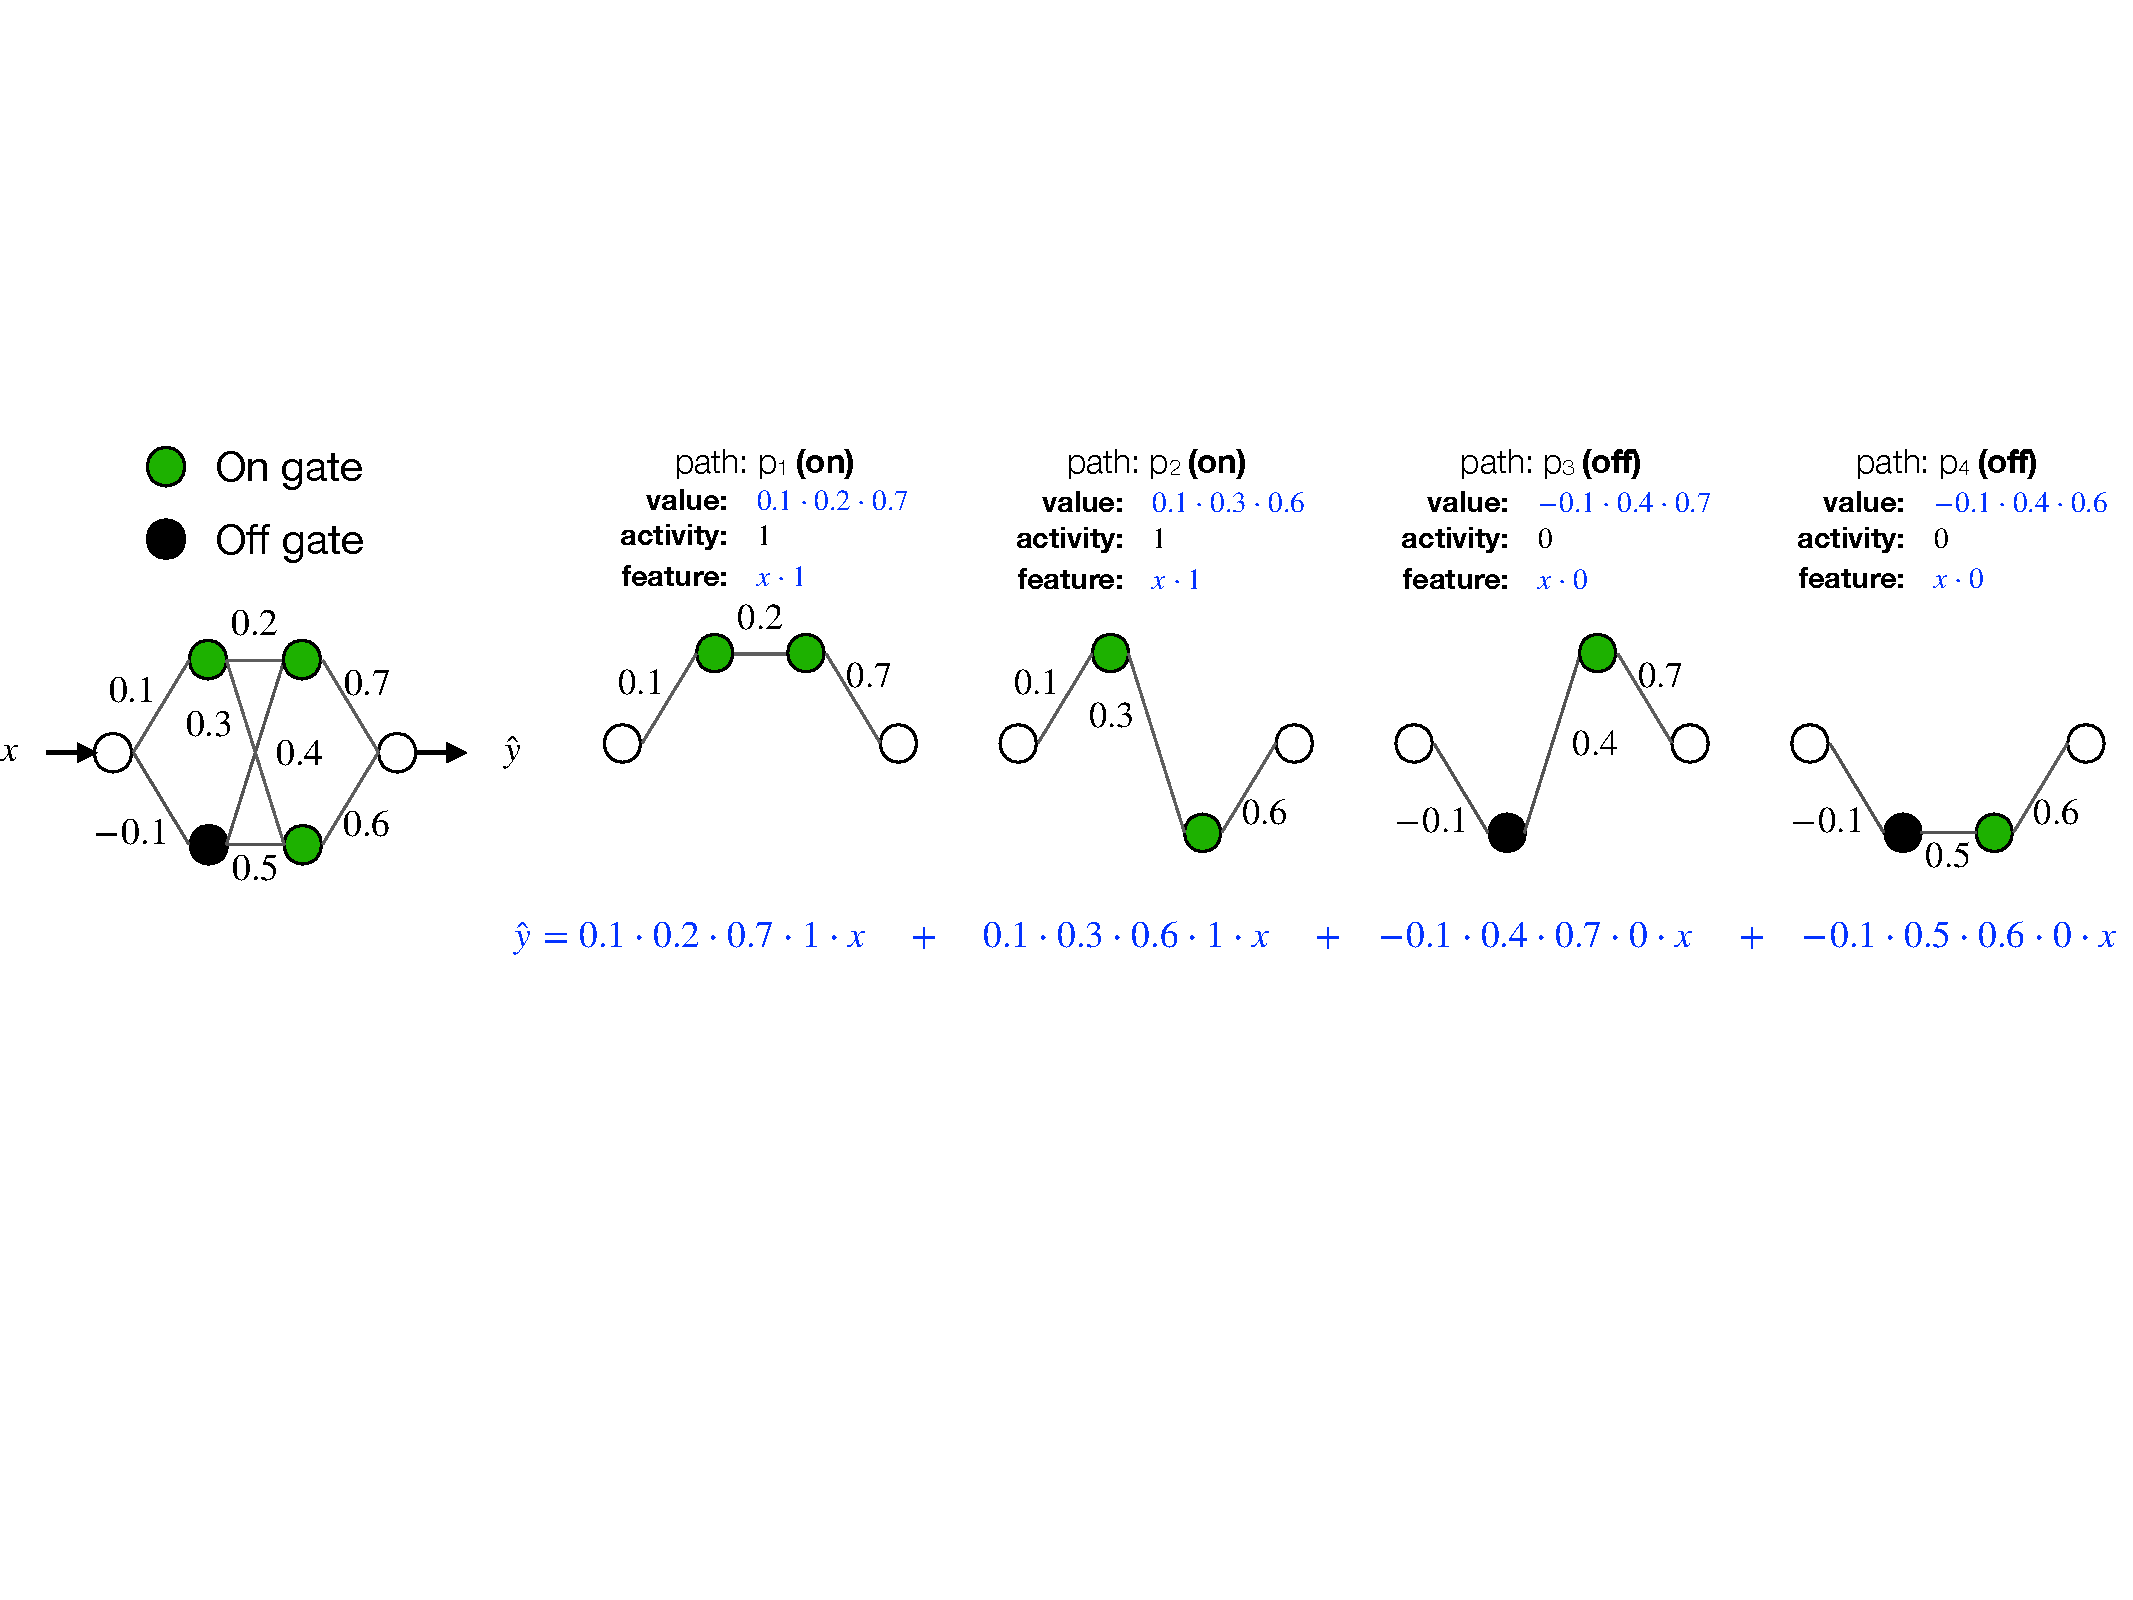
\includegraphics[scale=0.5]{figs/paths.pdf}
}
\caption{Illustration of \Cref{def:npf-npv} and \Cref{prop:npf-npv} in a  toy network with $2$ layers, $2$ gates per layer and $4$ paths. Paths $p_1$ and $p_2$ are `on' and paths $p_3$ and $p_4$ are `off'. The value, activity and feature of the individual paths are shown. $\hat{y}$ is the summation of the individual path contributions.}
\label{fig:paths}
\end{figure}

%\subsection{Overlap of Sub-Networks and Neural Path Kernel}
\begin{definition}[Overlap of active sub-networks]\label{def:overlap} 
The total number of `active' paths for both $x$ and $x'$ that pass through input node $i$ is defined to be:\\
{\centering{$\textbf{overlap}_{\Theta}(i,x,x') = \Lambda_{\Theta}(i,x,x') \eqdef \left|\{p\in[P]\colon  \Ifeat_0(p)=i, A_{\Theta}(x,p)= A_{\Theta}(x',p)=1\}\right|$}}
\end{definition}
%\subsection{NPK of FC-DNN: Product Kernel }
%\input{cnpkexample}
%\subsection{Neural Path Kernel : Similarity based on active sub-networks}
\begin{lemma}[Neural Path Kernel (NPK)]\label{lm:npk}
Let $D\in\R^{\din}$ be a vector of non-negative entries  and for $u,u'\in\R^{\din}$ , let $\ip{u,u'}_{D}=\sum_{i=1}^{\din}D(i)u(i)u'(i)$. Let $H_{\Theta}(x,x')\eqdef\langle\phi_{x,\Theta},\phi_{x',\Theta} \rangle$ be the neural path kernel (NPK). Then  
\begin{align*} 
\text{NPK}_{\Theta}(x,x')= H_{\Theta}(x,x')=\ip{x,x'}_{\Lambda_{\Theta}(\cdot,x,x')} 
\end{align*}
\end{lemma}
\textbf{Remark.} In the case of fully connected networks, $\textbf{overlap}_{\Theta}(i,x,x')$ is equal for all $i\in[\din]$, and hence $\text{NPK}_{\Theta}(x,x')=\ip{x,x'}\cdot\textbf{overlap}_{\Theta}(x,x')$.

\subsection{Deep Gated Network : Decoupling Gates (NPF) and Weights (NPV) }\label{sec:dgn}
\begin{comment}
\begin{wrapfigure}{r}{0.2\textwidth}
\centering
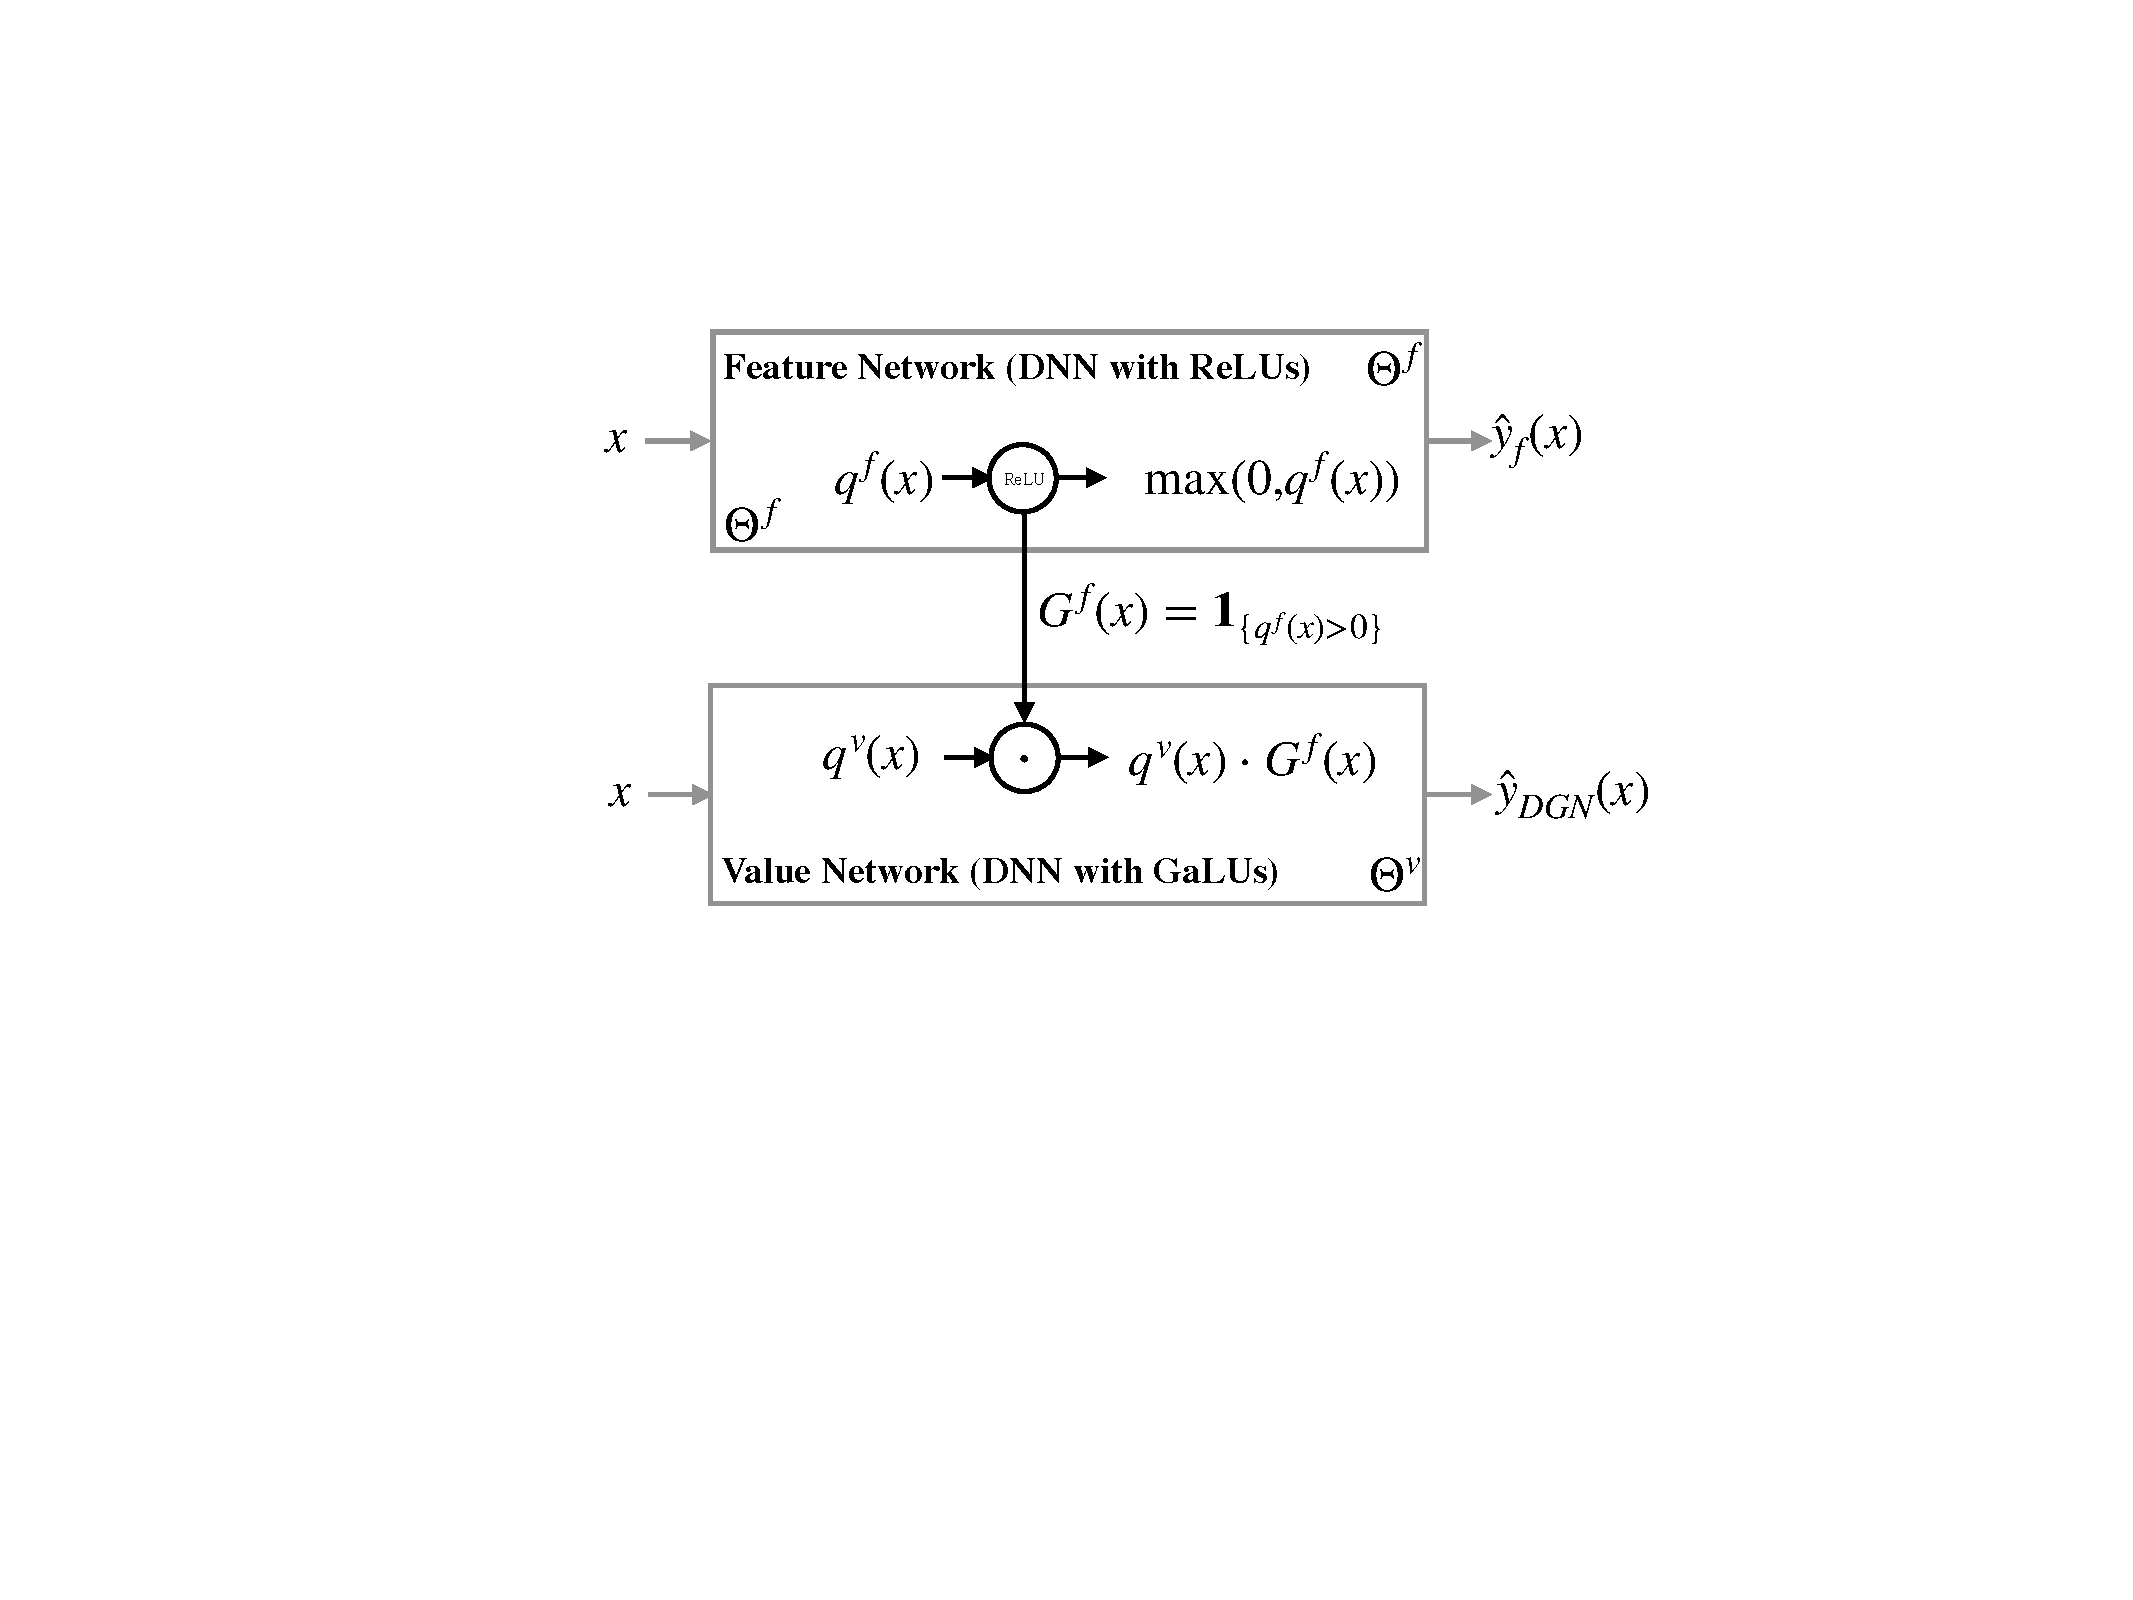
\includegraphics[scale=0.1]{figs/dgn-nips.pdf}
\caption{DGN}
\label{fig:dgn}
\end{wrapfigure}
\end{comment}

Since $\hat{y}_{\Theta}(x)=\ip{\phi_{x,\Theta},v_{\Theta}}$, during training, as $\Theta$ is learnt, both the NPFs and NPV are also learnt. To understand their roles better, $\phi_{x,\Theta}$ and $v_{\Theta}$ have to be separated.  This is achieved by the deep gated network (DGN) setup (see \Cref{fig:dgn}), which has two networks of \emph{identical architecture} namely the \emph{feature network} ($\Tf\in\R^{d^{\text{f}}_{\text{net}}}$) which holds the NPFs (i.e., the gating information) and the \emph{value network} ($\Tv\in\R^{d^{\text{v}}_{\text{net}}}$) which holds the NPV.  The combined parameterisation is denoted by $\Theta^{\text{DGN}}=(\Tf,\Tv)\in \R^{d^{\text{f}}_{\text{net}}+d^{\text{v}}_{\text{net}}}$.  The feature network is a DNN with ReLUs and the value network is a DNN with \emph{Gated Linear Units (GaLUs)} (terminology used in [\citenum{sss}]) whose output is the product of its pre-activation input $q^{\text{v}}(x)$and the external gating signal $G^{\text{f}}(x)$ (see \Cref{fig:dgn}). In \Cref{fig:dgn}, the main output of the DGN is $\hat{y}_{\text{DGN}}(x)$, while the other output $\hat{y}_{\text{f}}(x)$ is used to \emph{pre-train} the gates (see \Cref{sec:exp}).

\begin{figure}[h]
\begin{minipage}{0.38\columnwidth}
\resizebox{0.8\columnwidth}{!}{
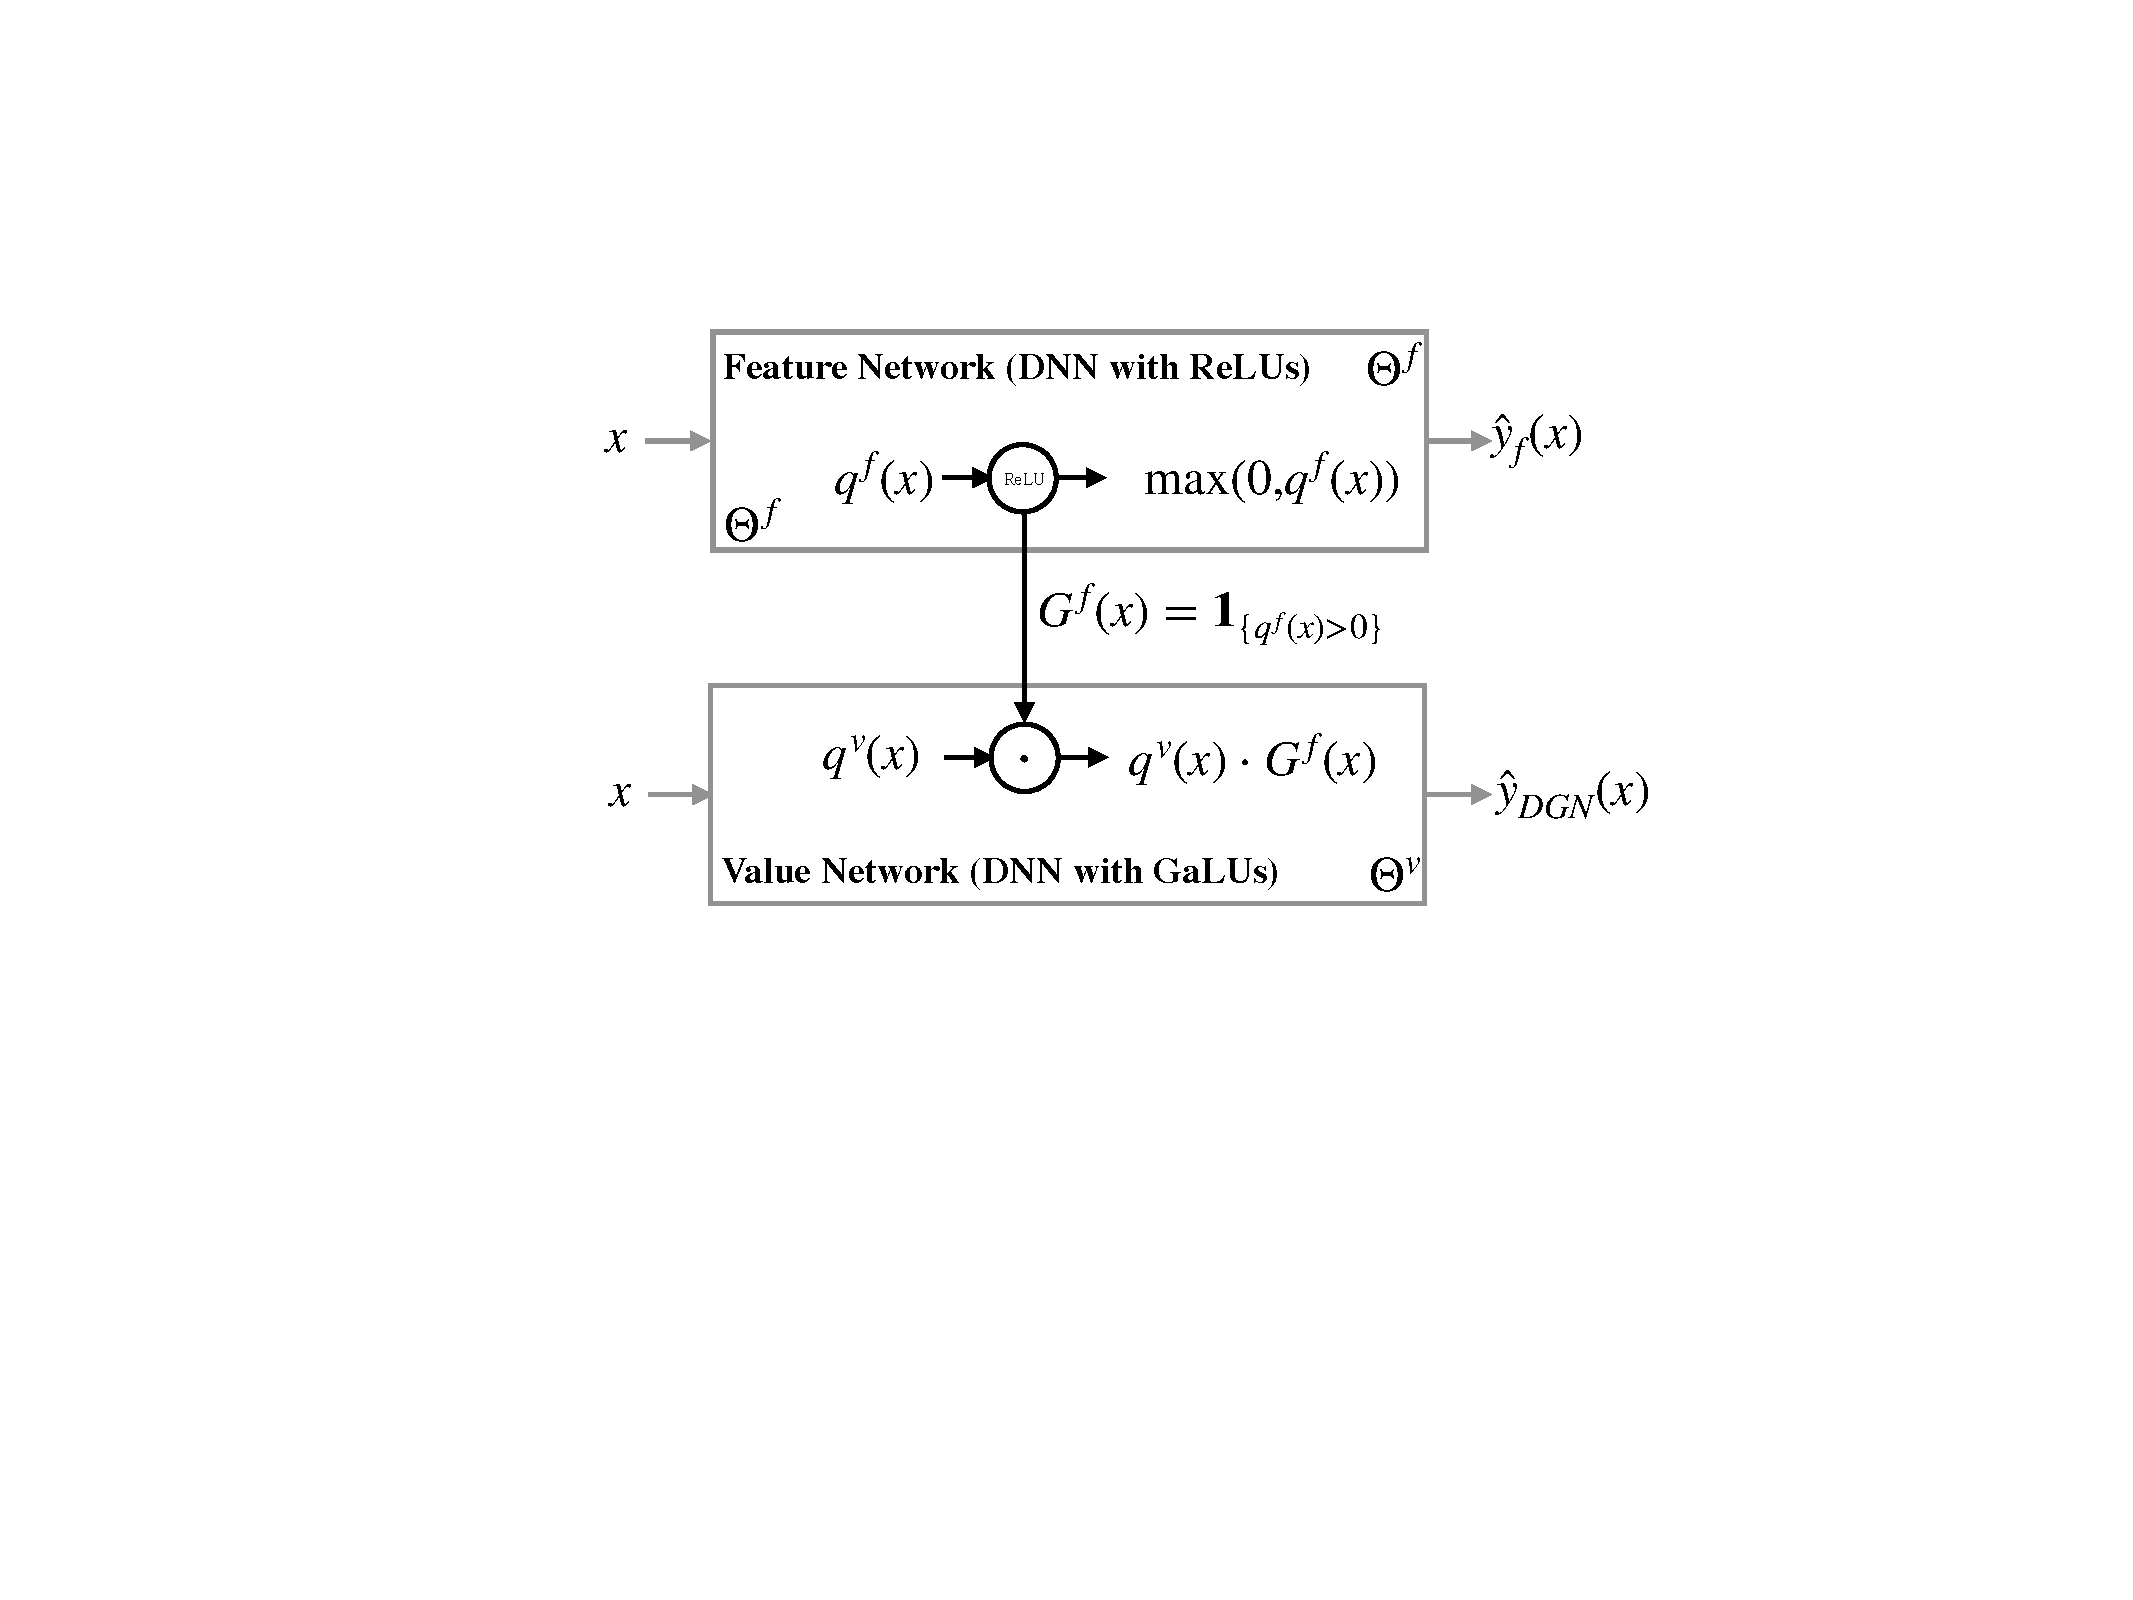
\includegraphics[scale=0.4]{figs/dgn-nips.pdf}
}
\caption{\small{Shows a DGN and interaction between two corresponding units, one in the feature and other in value network.}}
\label{fig:dgn}
\end{minipage}
\hfill
%\begin{flushright}
\begin{minipage}{0.55\columnwidth}
\begin{proposition}[{[\citenum{npk}]}]\label{prop:ntks} Let $\kv_{\Tdgn}(x,x')=\ip{ \nabla_{\Tv}\hat{y}_{\text{DGN}}(x), \nabla_{\Tv}\hat{y}_{\text{DGN}}(x')}$, and  $\kf_{\Tdgn}(x,x')=\ip{ \nabla_{\Tf}\hat{y}_{\text{DGN}}(x), \nabla_{\Tf}\hat{y}_{\text{DGN}}(x') }$ and $K_{\Tdgn}(x,x')$ be the NTK of the DGN. Then 
\begin{align*}
K_{\Tdgn}(x,x')=\kv_{\Tdgn}(x,x')+\kf_{\Tdgn}(x,x')
\end{align*}
\textbf{Remarks.} $\nabla_{\Tf}\hat{y}_{\text{DGN}}(x)$ flows via the feature network and $\nabla_{\Tv}\hat{y}_{\text{DGN}}(x)$ via the value network. Correspondingly there are two NTKs, i.e., $\kf$ and $\kv$. If the gates are fixed then, $\nabla_{\Tf}\hat{y}_{\text{DGN}}(x)=\mathbf{0}$ and $\kf_{\Tdgn}(x,x')=0$. 
\end{proposition}
%The deep gated network (DGN) setup (see \Cref{fig:dgn}), which has two networks namely the \emph{feature network} parameterised by $\Tf\in\R^{d^{\text{f}}_{\text{net}}}$ which holds the NPFs (i.e., the gating information) and a \emph{value network} parameterised by $\Tv\in\R^{d^{\text{v}}_{\text{net}}}$ which holds the NPV.  The combined parameterisation is denoted by $\Theta^{\text{DGN}}=(\Tf,\Tv)\in \R^{d^{\text{f}}_{\text{net}}+d^{\text{v}}_{\text{net}}}$.  
\end{minipage}
%\end{flushright}
\begin{comment}
\begin{minipage}{0.73\columnwidth}
\resizebox{\columnwidth}{!}{
\begin{tabular}{|ll|}\hline
Feature Network & Value Network\\
$z_{x,\Theta}(0)=x$& $z_{x,\Theta}(0)=x$ \\
$q_{x,\Theta}(i,l)=\sum_{j} \Theta(i,j,l)\cdot z_{x,\Theta}(j,l-1)$& $q_{x,\Theta}(i,l)=\sum_{j} \Theta(i,j,l)\cdot z_{x,\Theta}(j,l-1)$\\
$G_{x,\Theta}(i,l)=\mathbbm{1}_{\{q_{x,\Theta}(i,l)>0\}}$& $G_{x,\Theta}(i,l)=\mathbbm{1}_{\{q_{x,\Theta}(i,l)>0\}}$\\
$z_{x,\Theta}(i,l)=q_{x,\Theta}(i,l)\cdot G_{x,\Theta}(i,l)$ & $z_{x,\Theta}(i,l)=q_{x,\Theta}(i,l)\cdot G_{x,\Theta}(i,l)$ \\
 $\hat{y}_{\Theta}(x)=\sum_{j\in[w]} \Theta(1,j,d-1)\cdot z_{x,\Theta}(j,d-1)$ & $\hat{y}_{\Theta}(x)=\sum_{j\in[w]} \Theta(1,j,d-1)\cdot z_{x,\Theta}(j,d-1)$\\\hline
\end{tabular}
}
\end{minipage}
\end{comment}
\end{figure}

\begin{comment}
\subsection{NTK $\propto$ NPK}
\begin{assumption}\label{assmp:main}
(i) $\Tv_0$ is statistically independent of $\Tf_0$ (ii) $\Tv_0$ are i.i.d symmetric Bernoulli over $\{-{\sigma},+{\sigma}\}$. 
\end{assumption}

\begin{theorem}\label{th:main} Let $\sigma=\frac{\cscale}{\sqrt{w}}$. Under \Cref{assmp:main}, a $w\ra\infty$, for FC-DGN we have: 
\begin{align*}
\kv_{\Tdgn_0}(x,x') &\ra d\cdot \sigma^{d-1}\cdot H_{\Tf_0}(x,x')= d\cdot \sigma^{d-1}\cdot \ip{x,x'}_{\Lambda_{\Tf_0}(\cdot,x,x')}  \\
\end{align*}
\end{theorem}
\begin{figure}[h]
\begin{minipage}{0.49\columnwidth}
\centering
\resizebox{\columnwidth}{!}{
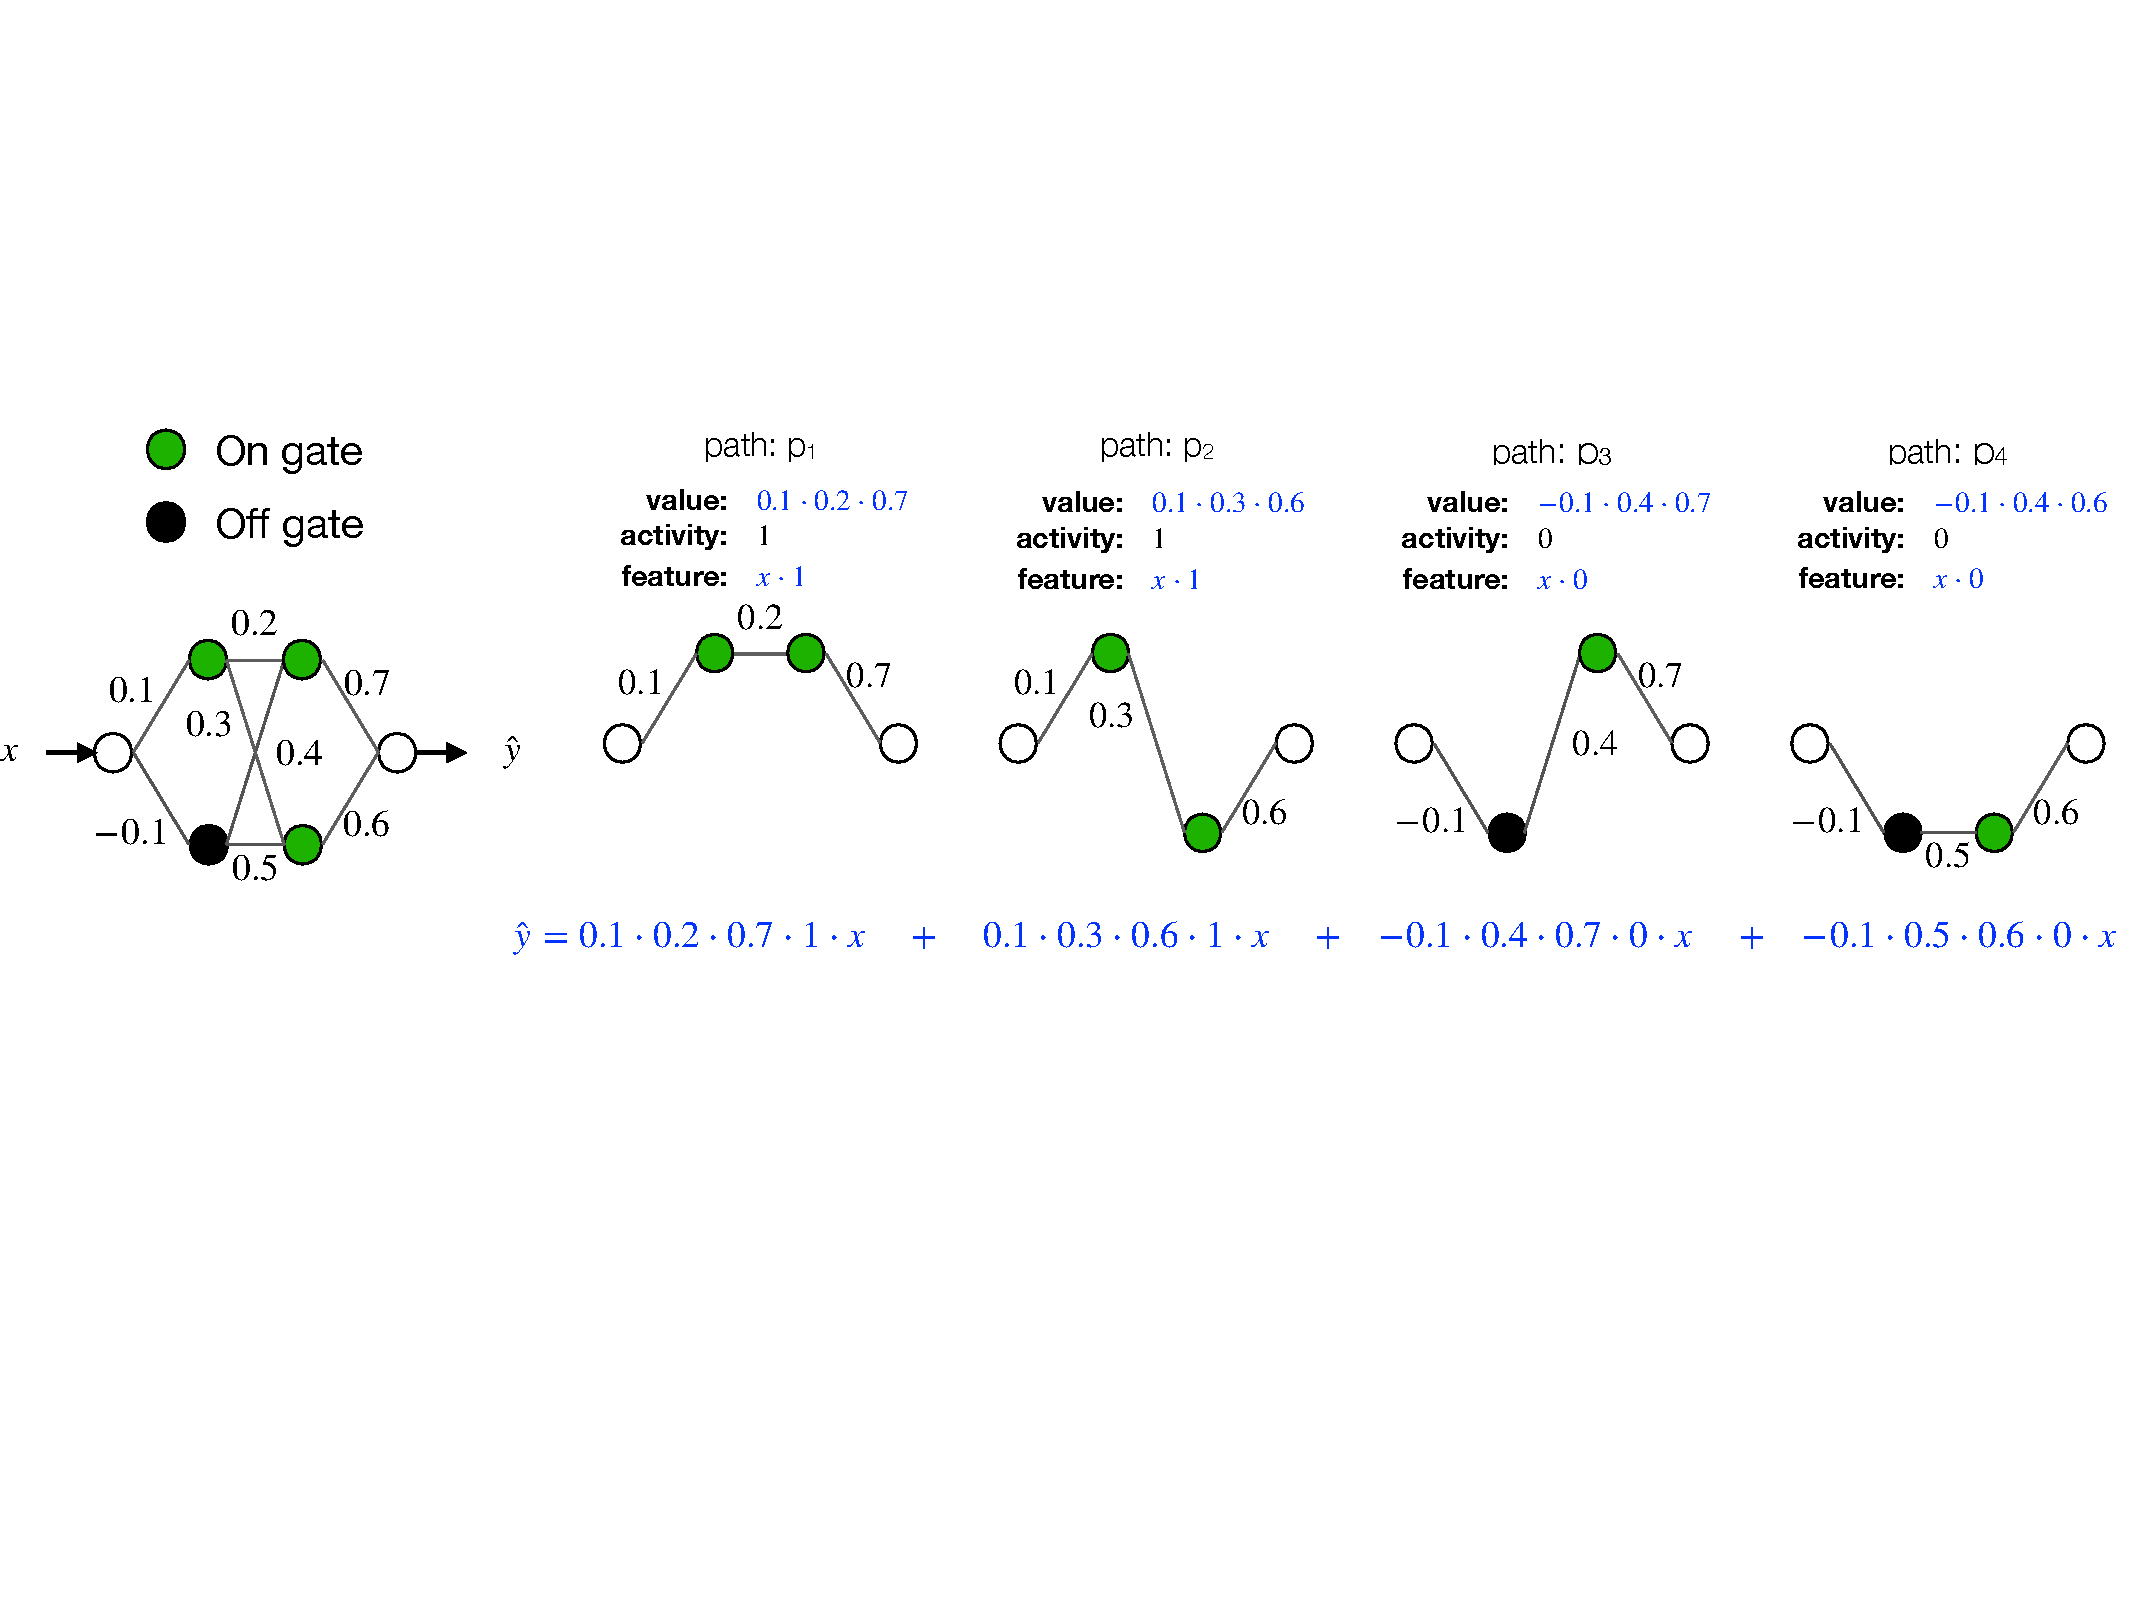
\includegraphics[scale=0.5]{figs/overlap.pdf}
}
\end{minipage}
\begin{minipage}{0.49\columnwidth}
\resizebox{\columnwidth}{!}{
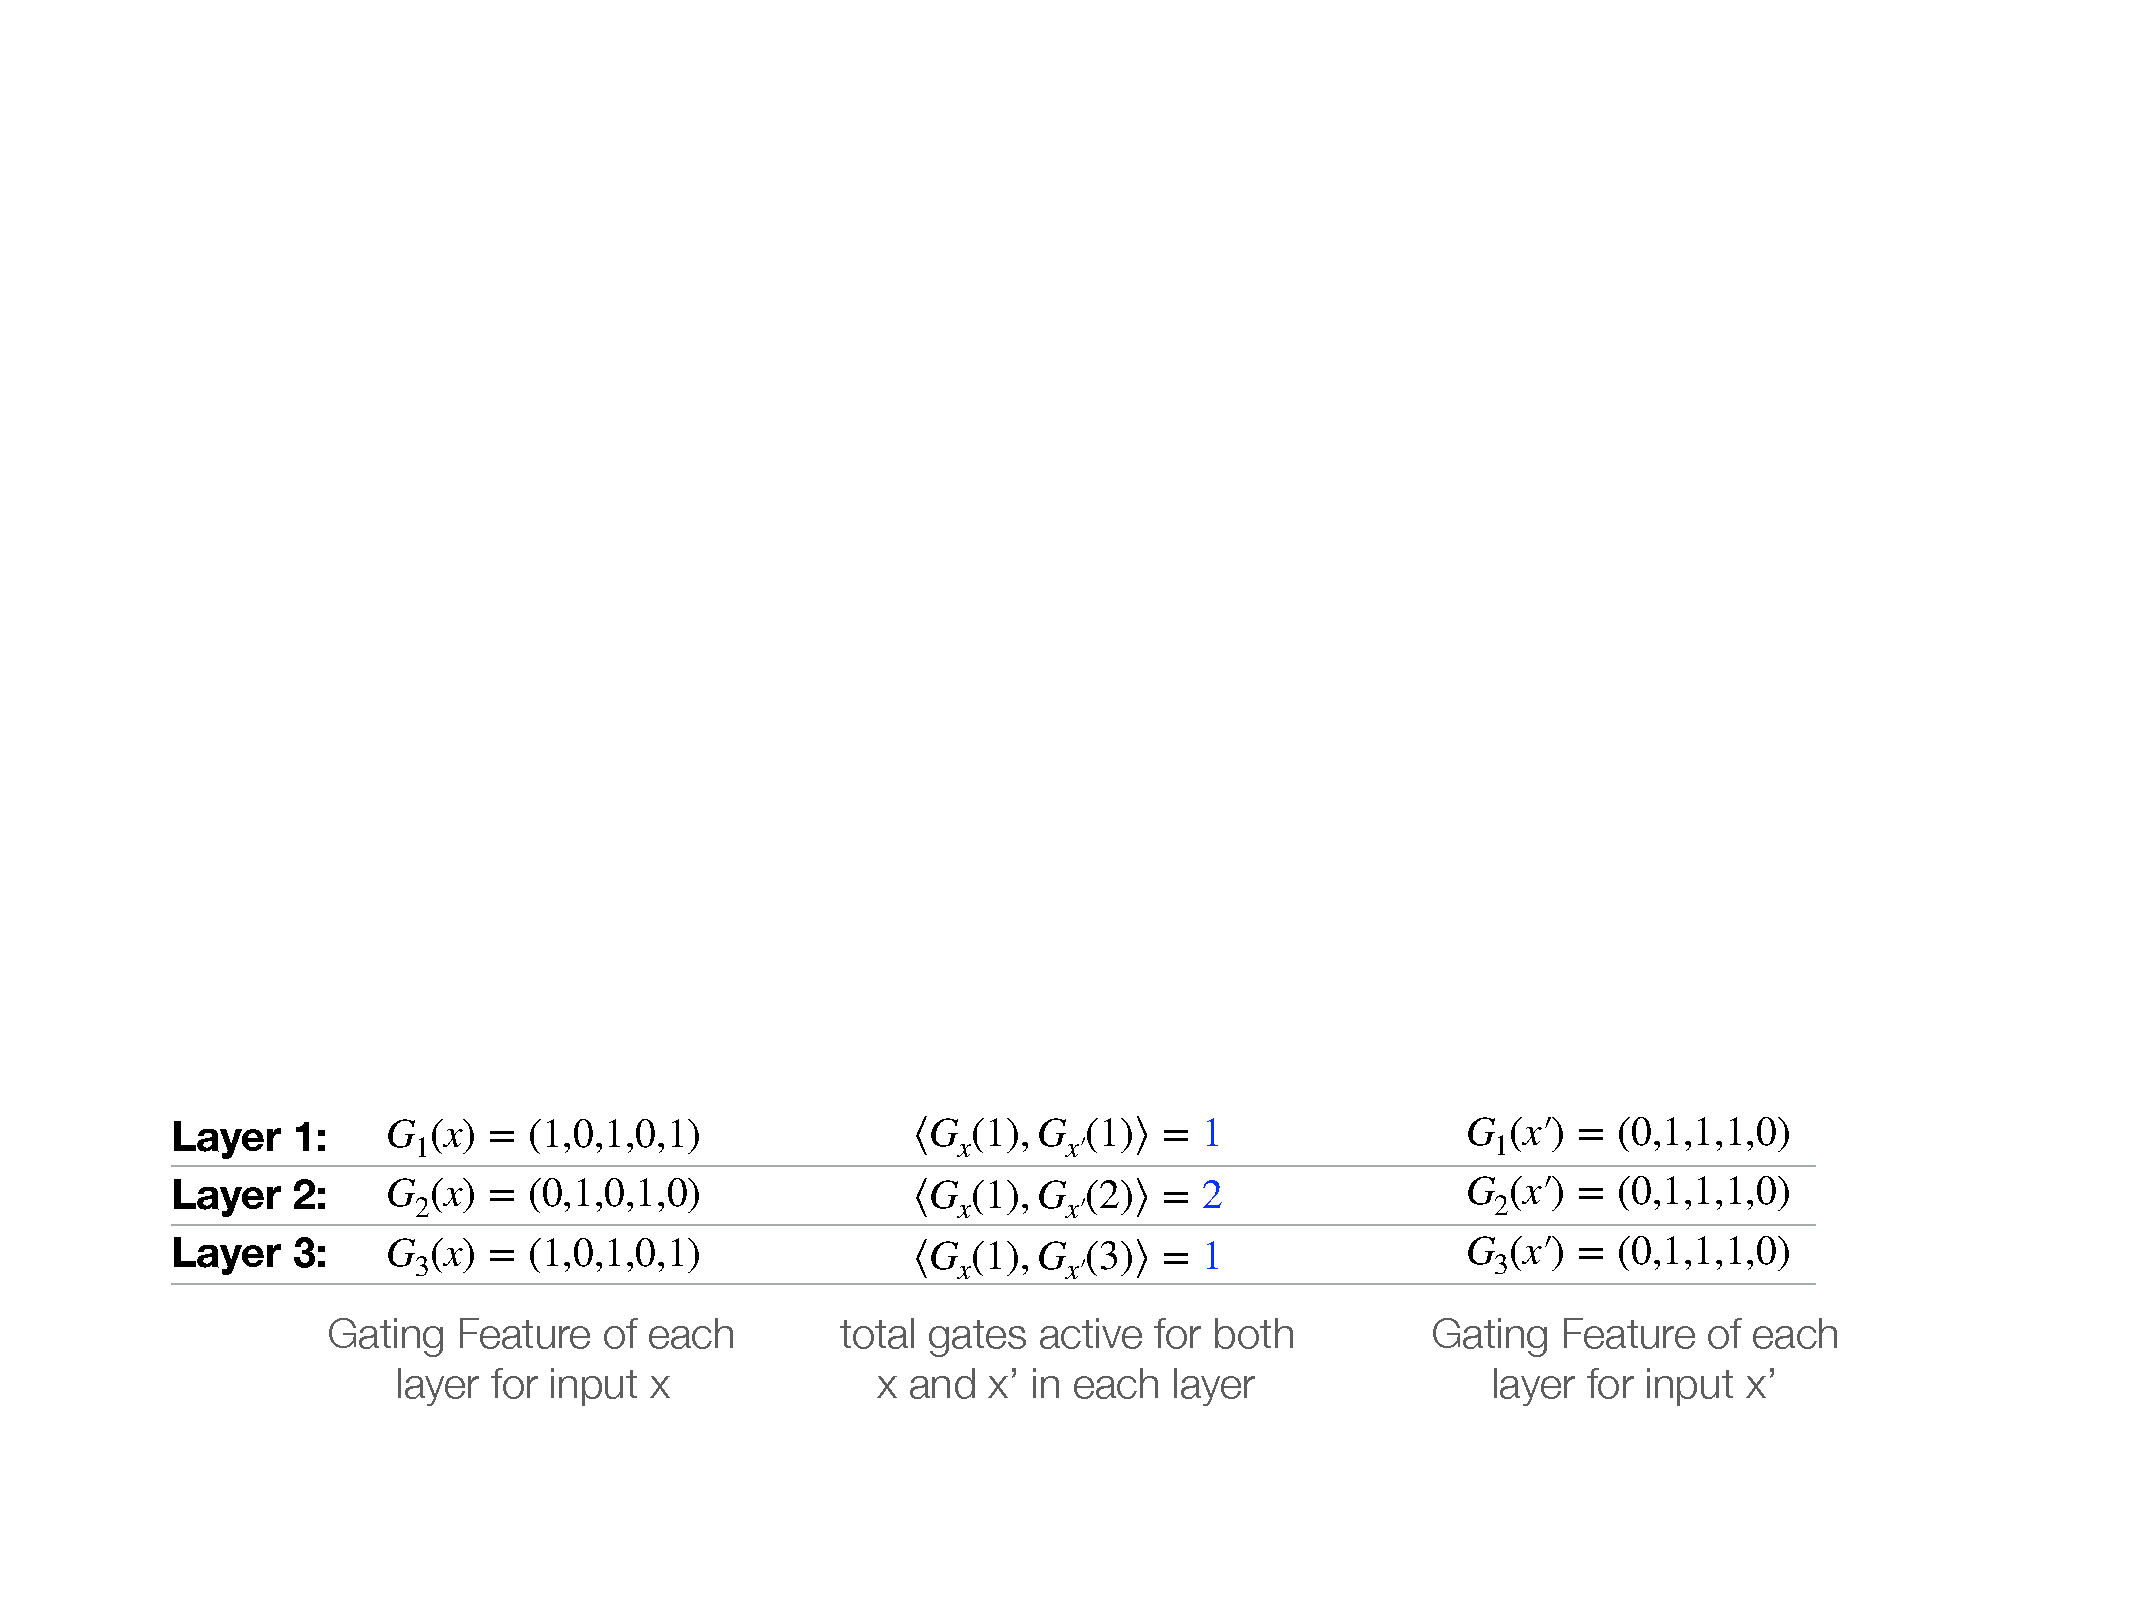
\includegraphics[scale=0.5]{figs/gating-features.pdf}
}
\end{minipage}
\caption{Shows a toy illustration of active sub-networks for two inputs $x$ and $x'$ and the common overlapping sub-network. The total number of active paths from any input node $i$, $\Lambda(i,x,')=\Pi_{i=1}^{3} \ip{G_l(x),G_l(x'}=1\cdot 2\cdot 1 =2$.}
\label{fig:overlap}
\end{figure}
\end{comment}
